\documentclass{article}
\usepackage{graphicx}
\usepackage{color} \usepackage{transparent}
\begin{document}

\title{Math-Based Optimization Language (MBOL)}

\author{Andrew Newell}

\maketitle

\tableofcontents

\section{Introduction}

This document should explain the MBOL language which is a subset of the Latex language. The goal is to convert natural mathematical representations of optimization programs into a solver. Currently MBOL supports linear programs or mixed integer programs.

\begin{figure}
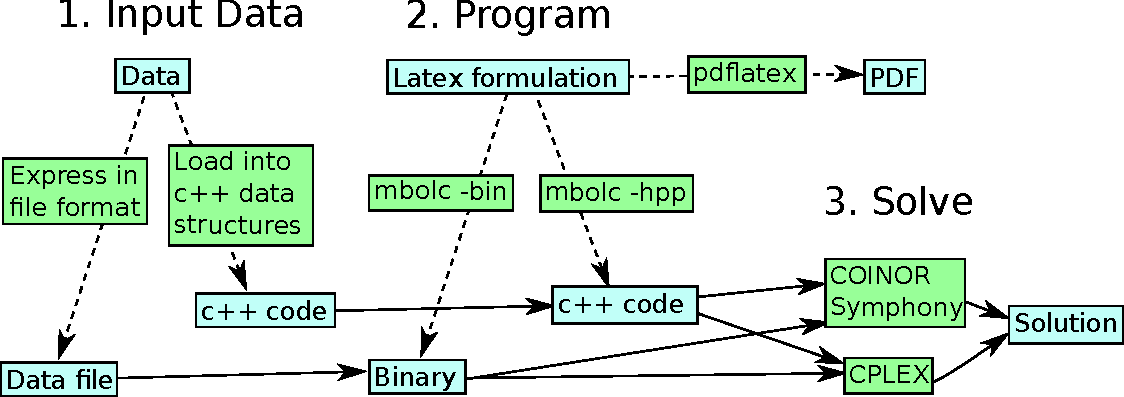
\includegraphics[width=\textwidth]{figures/mbol-overview.pdf}
\caption{Overview of workflow using MBOL}
\label{lab:overview}
\end{figure}

Figure~\ref{lab:overview} shows 

\section{Getting Started}

\section{MBOL Grammar Details}

\end{document}
